\subsection{Relations}
\label{sec:Suggestion:Relation}

The \textsf{Relation} part provides traceability links between \textsf{MM}
elements that are \textsf{changed}, and all \viewtype elements that are 
\textsf{impacted} by that change. One \textsf{MM} element
may impact several elements in the same \viewtype, but may also potentially
impact several \viewtypes. We only require so-called \emph{links}; richer
data structures for traceability may be used \autocite{Batot-Cabot-Gerard:2021}.

The way these traceability links are computed are left as implementation
details, and may happen in two ways: \emph{on-the-fly} whenever an \textsf{MM} element is evolved; and \emph{offline}
after a complete evolution session has terminated (based on diffing \autocite{Kehrer-Kelter-Taentzer:2011}, or using 
operation-based approaches \parencite{J:Lippe-Oosterom:1992}).

\begin{figure}[t]
    \centering
    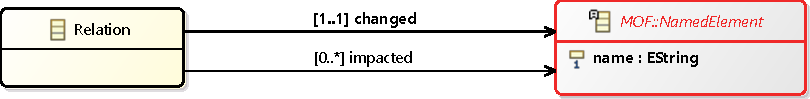
\includegraphics[width=\columnwidth]{Relation.pdf}
    \caption{Capturing \textsf{Relation}s between \textsf{MM} elements and \textsf{VT} elements.}
    \label{fig:Relation}
\end{figure}

In the \textsf{FSM} example associated to the \textsf{VT\_FSM},
we would have, among others, the following relations (with \textsf{Link}s noted 
as $\mathsf{<} \mathsf{changed} ; \mathsf{impacted} \mathsf{>}$):
\begin{itemize}
	\item Since computing the \textsf{name}s in \textsf{VT\_FSM} requires access
	to $\mathsf{Named \squaredots name}$, the following \textsf{Link}s would be
	created: 
	$\mathsf{<} \mathsf{Named \squaredots name} ; \mathsf{VT\_FSM \squaredots name} \mathsf{>}$;
	$\mathsf{<} \mathsf{Named \squaredots name} ; \mathsf{State \squaredots name} \mathsf{>}$;
	$\mathsf{<} \mathsf{Named \squaredots name} ; \mathsf{Transition \squaredots name} \mathsf{>}$.

	\item Creating an instance of \textsf{State} requires to take into account
	the value of $\mathsf{State \squaredots kind}$, which would produce the following
	\textsf{Link}s: 
	$\mathsf{<} \mathsf{State \squaredots kind} ; \mathsf{State} \mathsf{>}$;
	$\mathsf{<} \mathsf{State \squaredots kind} ; \mathsf{Initial} \mathsf{>}$;
	$\mathsf{<} \mathsf{State \squaredots kind} ; \mathsf{Regular} \mathsf{>}$.
	Depending on the precision of the traceability analysis, the following may
	eventually be produced as well: 
	$\mathsf{<} \mathsf{Kind \squaredots REGULAR} ; \mathsf{Regular} \mathsf{>}$ and
	$\mathsf{<} \mathsf{Kind \squaredots INITIAL} ; \mathsf{Initial} \mathsf{>}$.
	


	\item After Step 2, some \textsf{Link}s between the newly added attributes
	in $\mathsf{FSM \squaredots Transition}$ and the corresponding attributes in 
	$\mathsf{VT\_FSM \squaredots Transition}$ may be added as well. New 
	\textsf{Link}s taking into account the newly added literal in \textsf{Kind}
	would be added, similarly to the previous point.
\end{itemize}